%!TEX root = thesis.tex

\chapter{Results}

	In this chapter we will attempt to generalize step 3 of Friedgut by way of generalizing Friedgut's Lemma 6, Lemma 7, and Lemma 8. However, we will begin the chapter with some general lattice theory results that we will need later on in the chapter.

\section{Lattice Theory}

	We are not aware of any existing proofs of these lemmas, but some of them are fairly elementary and have a broad application, so they could have previously been proven by others.

	First we will prove, in three steps, that our inversion lattice remains a lattice when we enforce an order between two neighboring elements in the order. Recall from Definition \ref{lattice-definition} that in order to be a lattice the join and meet must exist for every pair of elements. Therefore Lemma \ref{identified-permutation-lattice-join} proves that the join exists, Lemma \ref{identified-permutation-lattice-meet} proves that the meet exists (with similar reasoning), and Proposition \ref{proposition-identification-is-lattice} combines both lemmas to prove that our structure is indeed still a lattice.

	\begin{lemma}
		\label{identified-permutation-lattice-join}
		Let $(Y, \le)$ be a poset and let $X = S(Y)$. Let $(X, \le_s)$ be a lattice, with $\le_s$ defined as in Definition \ref{partial-order-s-definition}. Let $\Inv$ be the inversion binary relation over $Y$ as defined in Definition \ref{inversion-definition}. Let $\join$ and $\join^{ij}$ denote the join in $(X, \le_s)$ and $(X^{ij}, \le^{ij}_s)$ respectively. Then for any $i,j \in Y$, if $i$ is either a direct successor or a direct predecessor of $j$ according to $\le_s$, it holds that for all $x, y \in X^{ij}$:
		\[
			\exists(x \join y) \implies \exists(x \join^{ij} y).
		\]
	\end{lemma}

	\begin{proof}
		Assume $\exists(x \join y)$. Let $z = x \join y$. Then $z$ is an upper bound of $\{x, y\}$:
		\[
			z \ge_s x \textrm{ and } z \ge_s y.
		\]
		And $z$ is the least upper bound of $\{x, y\}$. For every $a \in X$:
		\[
			(a \ge_s x \textrm{ and } a \ge_s y) \implies z \le_s a.
		\]
		Since $x \in X^{ij}$, then $(i, j) \notin Inv_x$. Since $z \ge_s x$, then $(i, j) \notin Inv_z$, so $z \in X^{ij}$. By definition $z \ge_s x \implies z \ge^{ij}_s x$ and $z \ge_s y \implies z \ge^{ij}_s y$. Therefore $z$ is an upper bound of $\{x, y\}$ in $X^{ij}$.

		For any $a \in X^{ij}$ if $a$ is an upper bound of $\{x, y\}$ in $X^{ij}$ then clearly $a$ is also an upper bound of $\{x, y\}$ in $X$. Therefore $z \le_s a$, so $z \le^{ij}_s a$, which means $z = x \join^{ij} y$. So clearly $x \join^{ij} y$ exists.
	\end{proof}

	\begin{lemma}
		\label{identified-permutation-lattice-meet}
		Let $Y$ be a set and let $X = S(Y)$. Let $(X, \le_s)$ be a lattice with $\le_s$ defined as above. Let $\Inv$ be the inversion binary relation over $Y$ as defined above. Let $\meet$ and $\meet^{ij}$ denote the meet in $(X, \le_s)$ and $(X^{ij}, \le^{ij}_s)$ respectively. Then for any $i,j \in Y$, if $i$ is either a direct successor or a direct predecessor of $j$ according to $\le_s$, it holds that for all $x, y \in X^{ij}$:
		\[
			\exists(x \meet y) \implies \exists(x \meet^{ij} y).
		\]
	\end{lemma}

	\begin{proof}
		Assume $\exists(x \meet y)$. Let $z = x \meet y$. Then $z$ is a lower bound of $\{x, y\}$:
		\[
			z \le_s x \textrm{ and } z \le_s y.
		\]
		And $z$ is the greatest lower bound of $\{x, y\}$: for every $a \in X$:
		\[
			(a \le_s x \textrm{ and } a \le_s y) \implies z \ge_s a.
		\]

		We will now detour to show that $z \in X^{ij}$. Since $z = x \meet y$, then $\Inv_z = (\Inv_x \cup \Inv_y)^t$ \cite{markowsky1994permutation}. Because $x,y \in X^{ij}$ we know that $(i, j) \notin (\Inv_x \cup \Inv_y)$. Therefore, in order to have $(i, j) \in (\Inv_x \cup \Inv_y)^t$ we would need to have $(i, k) \in \Inv_x$ and $(k, j) \in \Inv_y$ for any $k \in Y$, which is impossible because $i$ is either a direct successor or a direct predecessor of $j$. Therefore $(i, j) \notin Inv_z$, so $z \in X^{ij}$.

		By definition $z \le_s x \implies z \le^{ij}_s x$ and $z \le_s y \implies z \le^{ij}_s y$. Therefore $z$ is a lower bound of $\{x, y\}$ in $X^{ij}$.

		For any $a \in X^{ij}$ if $a$ is a lower bound of $\{x, y\}$ in $X^{ij}$ then clearly $a$ is also a lower bound of $\{x, y\}$ in $X$. Therefore $z \ge_s a$, so $z \ge^{ij}_s a$, which means $z = x \meet^{ij} y$. So clearly $x \meet^{ij} y$ exists.
	\end{proof}

	\begin{proposition}
		\label{proposition-identification-is-lattice}
		Let $Y$ be a set and let $X = S(Y)$. Let $(X, \le_s)$ be a lattice with $\le_s$ defined as above. Let $\Inv$ be the inversion binary relation over $Y$ as defined above. Then for any $i,j \in Y$, if $i$ is either a direct successor or a direct predecessor of $j$ according to $\le_s$, it holds that $(X^{ij}, \le^{ij}_s)$ is a lattice.
	\end{proposition}

	\begin{proof}
		We know that $\exists(x \join y)$ and $\exists(x \meet y)$ because $(X, \le_s)$ is a lattice. Therefore by Lemma \ref{identified-permutation-lattice-join} and Lemma \ref{identified-permutation-lattice-meet} we have $\exists(x \join^{ij} y)$ and $\exists(x \meet^{ij} y)$ respectively. So $(X^{ij}, \le^{ij}_s)$ is a lattice, by definition of a lattice.
	\end{proof}

	Now we will show that a ``grid'' of lattices is also a lattice. For example, suppose we have the lattice in Figure \ref{figure-one-dimensional-lattice}. The top element is the greatest, and the arrows show the ``less than'' relationship between elements. Each column of numbers represents a ranking of alternatives ${1, 2, 3}$ in which we don't care about the relationship between alternative $1$ and $2$ so we simply replace alternative $2$ with $1$ in the ranking. All this aside though, this proof is valid for any lattice.

	\begin{figure}[ht]
		\begin{center}
			\includegraphics[width=1in]{../figures/diagram5.pdf}
			\caption{A single dimension of lattice.}
			\label{figure-one-dimensional-lattice}
		\end{center}
	\end{figure}

	If we were to make that lattice into a 2-dimensional ``grid'' it would look like Figure \ref{figure-two-dimensional-lattice}. This would be the case if we only had two voters ($n = 2$).

	\begin{figure}[ht]
		\begin{center}
			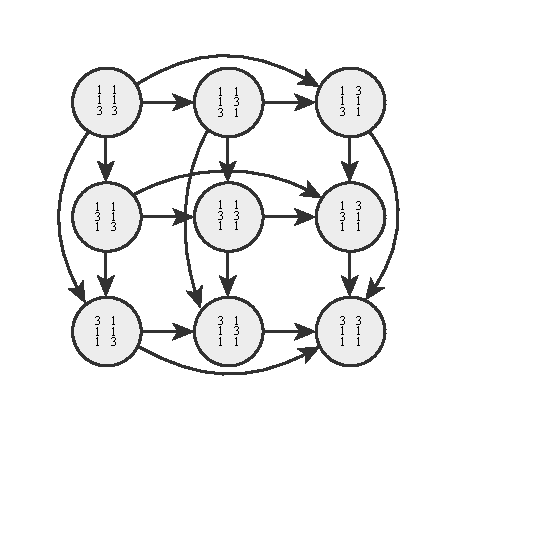
\includegraphics[width=3in]{../figures/diagram6.pdf}
			\caption{A 2-dimensional version of the lattice from Figure \ref{figure-one-dimensional-lattice}.}
			\label{figure-two-dimensional-lattice}
		\end{center}
	\end{figure}

	\begin{proposition}
		\label{proposition-grid-is-lattice}
		Let $(X, \le)$ be a lattice. Let $X^n$ be the set of all $n$-tuples of elements of $X$. Let $\le^n$ be defined as: for all $x, y \in X$ and all $i \in \{1, \ldots, n\}$
		\[
			x \le^n y \iff x_i \le y_i.
		\]
		Then $(X^n, \le^n)$ is a lattice.
	\end{proposition}

	\begin{proof}
		By definition of a lattice, $(X^n, \le^n)$ is a lattice if for any two elements $s, t \in S^n$, $s \join t$ exists and $s \meet t$ exists.

		First we show that $s \join t$ exists. We define $u \in X^n$ such that $u_i = s_i \join t_i$, $\forall i \in \{1, \ldots, n\}$, and we show that $u = s \join t$. Because $u_i = s_i \join t_i$, we have
		\[
			u_i \ge s_i \textrm{ and } u_i \ge s_i
		\]
		so
		\[
			u \ge^n s \textrm{ and } u \ge^n t
		\]
		meaning that $u$ is an upper bound for $s$ and $t$. Suppose there is some $v \in X^n$ which is also an upper bound for $s$ and $t$. Then $\forall i \in \{1, \ldots, n\}$ we have
		\[
			v_i \ge s_i \textrm{ and } v_i \ge t_i
		\]
		so since $u_i = s_i \join t_i$, then $u_i \le v_i$. Therefore $u \le^n v$, i.e. $u$ is the least upper bound of $\{s, t\}$.

		Second we show that $s \meet t$ exists (by the same argument). We define $u \in X^n$ such that $u_i = s_i \meet t_i$, $\forall i \in \{1, \ldots, n\}$, and we show that $u = s \meet t$. Because $u_i = s_i \meet t_i$, we have
		\[
			u_i \le s_i \textrm{ and } u_i \le s_i
		\]
		so
		\[
			u \le^n s \textrm{ and } u \le^n t
		\]
		meaning that $u$ is a lower bound for $s$ and $t$. Suppose there is some $v \in X^n$ which is also a lower bound for $s$ and $t$. Then $\forall i \in \{1, \ldots, n\}$ we have
		\[
			v_i \le s_i \textrm{ and } v_i \le t_i
		\]
		so since $u_i = s_i \meet t_i$, then $u_i \ge v_i$. Therefore $u \ge^n v$, i.e. $u$ is the greatest lower bound of $\{s, t\}$.
	\end{proof}


\section{Main Theorem}

	Friedgut's main theorem is proved in three steps; the first two are already generalized. Therefore to generalize the main theorem we need only generalize the third step. This step is comprised of Lemma 6, Lemma 7, and Lemma 8 which we will generalize one at a time. Therefore, Step 3 of Friedgut is our main theorem:

	\begin{theorem}[Lemma 3 of Friedgut]
		For every SCF $f$ on $m$ alternatives and every $a, b \in C$:
		\[
			M^{a, b}(f) \le m! \cdot \sum_i M_i(f)
		\]
	\end{theorem}

	For the rest of the proof we will fix a SCF $f$.


\section{Generalized Lemma 6 of Friedgut}

	For any preference profile $p \in P$ there are $(\frac{m!}{2})^n$ profiles $x$ such that $x|_{\{a, b\}} = p|_{\{a, b\}}$. This is because there are $m!$ possible preference lists; half of them will have the preference between $a$ and $b$ that agrees with $p|_{\{a, b\}}$ and half will disagree. For each voter this gives $\frac{m!}{2}$ possible preference lists which gives $(\frac{m!}{2})^n$ profiles comprised of these preference lists.

	\begin{definition}
		Let $C$ be a set of alternatives. Let $a, b, c \in C$ be any three alternatives. Let $p \in L(C)^n$ be a preference profile for $n$ voters, and let $f$ be a SCF. We define
		\[
			A^{a,b}_c(p) = \{x \in L(C)^n \mid x|_{\{a,b\}} = p|_{\{a,b\}}, f(x) = c\}
		\]
	\end{definition}

	Therefore we can rewrite $M^{a,b}(f)$ as follows.

	\begin{lemma}[Lemma 6 of Friedgut]
		\label{friedgut-lemma-6}
		Let $C$ be a set of alternatives. Let $a, b \in C$ be any two alternatives. Let $m = |C|$ and let $n$ be the number of voters. Let $f$ be a SCF. We have
		\[
			M^{a,b}(f) = E_{p \in L(C)^n} \left[ \frac{|A^{a,b}_a(p)|}{\left(\frac{m!}{2}\right)^n} \cdot \frac{|A^{a,b}_b(p)|}{\left(\frac{m!}{2}\right)^n} \right]
		\]
	\end{lemma}

	\begin{proof}
		This is just a rewording of the definition of $M^{a,b}(f)$.
	\end{proof}


\section{Generalized Lemma 7 of Friedgut}

	We now attempt to relate $M_i(f)$ to $A$.

	Let $n$ be the number of voters. Let $C = \{1, \ldots, m\}$ be a set of alternatives, and let $a,b \in C$ be any two alternatives. We define an anonymized version of the alternatives as $C' = \{c_1, \ldots, c_m\}$, totally ordered as $c_1 < \ldots < c_m$.

	\begin{definition}
		$C'$ is isomorphic to $C$ and we define the mapping function $g^{a,b} : C \to C'$ such that
		\begin{align*}
			g^{a,b}(x) =
			\begin{cases}
				c_x & \textrm{if } x \in C \backslash \{1, 2, a, b\} \\
				c_1 & \textrm{if } x = a \\
				c_2 & \textrm{if } x = b \\
				c_a & \textrm{if } x = 1 \\
				c_b & \textrm{if } x = 2
			\end{cases}
		\end{align*}
		We define $G^{a,b} : L(C) \to L(C')$ such that
		\[
			G^{a,b}(x) = (g^{a,b}(x_1), \ldots, g^{a,b}(x_m))
		\]
	\end{definition}

	\begin{definition}
		We define the partial ordering, $\le^G_s$, on $L(C)$ such that for all $x, y \in L(C)$:
		\[
			x \le^G_s y \iff G^{a,b}(x) \le_s G^{a,b}(y)
		\]
		where $\le_s$ is defined in Definition \ref{partial-order-s-definition}.
	\end{definition}

	Clearly $(L(C), \le^G_s)$ is a lattice, because it is isomorphic to $(L(C), \le_s)$ which is a lattice.

	\begin{definition}
		We define the partial order $(\le^G_s)^n$ on $L(C)^n$ such that for all $x,y \in L(C)^n$ and all $i \in \{1, \ldots, n\}$:
		\[
			x (\le^G_s)^n y \iff x_i \le^G_s y_i
		\]
	\end{definition}

	We have that $(L(C)^n, (\le^G_s)^n)$ is a lattice by Proposition \ref{proposition-grid-is-lattice} and the fact that $(L(C), \le^G_s)$ is a lattice.

	\begin{definition}
		Let $p \in L(C)^n$. We define the \emph{upper edge border} of $A^{a,b}_a(p)$, denoted $\partial A^{a,b}_a(p)$, to be the set of directed edges whose tail is in $A^{a,b}_a(p)$ and whose head is not in $A^{a,b}_a(p)$. Formally, for all $i \in \{1, \ldots, n\}$:
			\[
				\partial_i A^{a,b}_a(p) = \{ (x_{-i}, x_i, x'_i) \mid (x_{-i}, x_i) \in A^{a,b}_a(p), (x_{-i}, x'_i) \notin A^{a,b}_a(p), x_i <^G_s x'_i \}
			\]
		and
			\[
				\partial A^{a,b}_a(p) = \bigcup_j \partial_j A^{a,b}_a(p)
			\]
		We define the upper edge border of $A^{a,b}_b(p)$ analogously.
	\end{definition}

	\begin{lemma}
		\label{manipulation-per-edge-in-a}
		Let $p, p' \in L(C)^n$ be profiles such that for all $i \in \{1, \ldots, n\}$:
		\begin{align*}
			p_{-i} &= p'_{-i} \textrm{ and} \\
			p_i|_{a,b} &= p'_i|_{a,b}
		\end{align*}
		If either
		\begin{align*}
			(x_{-i}, x_i, x'_i) &\in \partial_i A^{a,b}_a(p) \textrm{ or} \\
			(x_{-i}, x_i, x'_i) &\in \partial_i A^{a,b}_b(p)
		\end{align*}
		then the pair $p, p'$ corresponds to at least one successful manipulation.
	\end{lemma}

	\begin{proof}
		By definition of the upper edge border we have
		\[
			x_i \le^G_s x'_i
		\]
		And by definition of $A^{a,b}_a$ and $A^{a,b}_b$ we have
		\[
			x_i|_{\{a,b\}} = x'_i|_{\{a,b\}}
		\]

		For $(x_{-i}, x_i, x'_i) \in \partial_i A^{a,b}_a(p)$, we know that $f((x_{-i}, x_i)) = a$ and $f((x_{-i}, x'_i)) = t$ for $t \in C \backslash \{a\}$. If $t \succ_{x_i} a$ then $x'_i$ is a successful manipulation of $(x_{-i}, x_i)$. Otherwise, $a \succ_{x_i} t$. If this is the case, then we know that $(a, t) \notin Inv_{x_i}$, and because $x_i \le^G_s x'_i$ we have $(a, t) \notin Inv_{x'_i}$, which means $a \succ_{x'_i} t$. Therefore $x_i$ is a successful manipulation of $(x_{-i}, x'_i)$.

		And analogously for $(x_{-i}, x_i, x'_i) \in \partial_i A^{a,b}_b(p)$, either $x'_i$ is a successful manipulation of $(x_{-i}, x_i)$ or $x_i$ is a successful manipulation of $(x_{-i}, x'_i)$.
	\end{proof}

	\begin{lemma}[Lemma 7 of Friedgut]
		\label{friedgut-lemma-7}
		\[
			M_i(f) \ge \frac{1}{m!} \left(\frac{m!}{2}\right)^{-n} E_x \left[|\partial_i A^{a,b}_a(p)| + |\partial_i A^{a,b}_b(p)| \right]
		\]
	\end{lemma}

	\begin{proof}
		Recall the definition of $M_i(f)$: given a profile $p \in P$ and vote $p'_i \in V$ chosen uniformly at random, $M_i(f)$ is the probability that $p'_i$ is a successful manipulation of $p$ by voter $i$. Therefore to lower bound $M_i(f)$ we start with $p$ and $p'_i$ chosen uniformly at random. We can think of these as two distinct profiles, $p$ and $p'$, where $p' = (p_{-i}, p'_i)$.

		Clearly $p_{-i}|_{\{a,b\}} = p'_{-i}|_{\{a,b\}}$, but we will have $p_i|_{\{a,b\}} = p'_i|_{\{a,b\}}$ only with probability $\frac{1}{2}$, and we condition the following on this being the case. So we have $p|_{\{a,b\}} = p'|_{\{a,b\}}$.

		By Lemma \ref{manipulation-per-edge-in-a}, each $(x_{-i}, x_i, x'_i) \in (\partial_i A^{a,b}_a(p) \cup \partial_i A^{a,b}_b(p))$ corresponds to at least one successful manipulation. Note that if $(x_{-i}, x_i, x'_i) \in \partial_i A^{a,b}_a(p)$ then $(x_{-i}, x'_i, x_i) \notin \partial_i A^{a,b}_a(p)$.

		Therefore we can lower bound $M_i(f)$ by the probability that an edge is in either $\partial_i A^{a,b}_a(p)$ or $\partial_i A^{a,b}_b(p)$. The total possible number of edges is
		\[
			\frac{m!}{2} \cdot \frac{m!}{2} \cdot \left(\frac{m!}{2}\right)^{n-1} = \frac{m!}{2}\left(\frac{m!}{2}\right)^{n}
		\]
		So the probability that a randomly chosen edge is in either $\partial_i A^{a,b}_a(p)$ or $\partial_i A^{a,b}_b(p)$ is
		\[
			\frac{2}{m!} \left(\frac{2}{m!}\right)^{n} \cdot E \left[ |\partial_i A^{a,b}_a(p)| + |\partial_i A^{a,b}_b(p)| \right]
		\]
		Note that we can sum the probabilities for $\partial_i A^{a,b}_a(p)$ and $\partial_i A^{a,b}_b(p)$ because they are disjoint by the definition of the upper edge border; an edge cannot satisfy both $(x_{-i}, x_i) \in A^{a,b}_a(p)$ and $(x_{-i}, x_i) \in A^{a,b}_b(p)$ simultaneously because if $f((x_{-i}, x_i)) = a$ then $f((x_{-i}, x_i)) \ne b$ and vice versa.

		We conditioned our analysis on $p_i = p'_i$, so then, our lower bound becomes
		\[
			M_i(f) \ge \frac{1}{2} \cdot \frac{2}{m!}\left(\frac{2}{m!}\right)^{n} \cdot E \left[ |\partial_i A^{a,b}_a(p)| + |\partial_i A^{a,b}_b(p)| \right]
		\]
		And simplified
		\[
			M_i(f) \ge \frac{1}{m!}\left(\frac{2}{m!}\right)^{n} \cdot E \left[ |\partial_i A^{a,b}_a(p)| + |\partial_i A^{a,b}_b(p)| \right]
		\]
	\end{proof}

	Summing over $i$ we get

	\begin{corollary}[Corollary 1 of Friedgut]
		\[
			\frac{1}{m!} \cdot \left(\frac{m!}{2}\right)^{-n} E_p[|\partial A^{a,b}_a(p)| + |\partial A^{a,b}_b(p)|] \le \sum_i M_i(f)
		\]
	\end{corollary}


\section{Generalized Lemma 8 of Friedgut}

	In this section we will fix candidates $a, b$ and profile $p$, and for the sake of readability we will define the following.

	First, we revise our previous definition to allow us to limit $A$ and $B$ to a specific set of lattice nodes, here referred to as $X$:
	\begin{align*}
		A^{a,b}_c(p, X) = \{x \in X \mid x|_{\{a,b\}} = p|_{\{a,b\}}, f(x) = c\}
	\end{align*}

	Next we define shorthand for $A$ and $B$:
	\begin{align*}
		A(X) &= A^{a,b}_a(p, X) \\
		B(X) &= A^{a,b}_b(p, X) \\
	\end{align*}
	and when we refer to $A$ and $B$ without parameters, we assume they are only limited to valid profiles:
	\begin{align*}
		A &= A(V^n) \\
		B &= B(V^n) \\
	\end{align*}

	We also rename the orderings:
	\begin{align*}
		\le &\textrm{ is } \le_s^G \\
		\le^n &\textrm{ is } (\le_s^G)^n \\
	\end{align*}

	And finally, we recall $(V^n, \le^n)$ is our $n$-dimensional lattice, and that $A$ and $B$ reside in this space:
	\begin{align*}
		A &\subseteq V^n \\
		B &\subseteq V^n \\
	\end{align*}

	\begin{lemma}[Lemma 8 of Freidgut]
		\label{friedgut-lemma-8}
		For every disjoint $A, B$ we have that
		\[
			|\partial A| + |\partial B| \ge \left( \frac{2}{m!} \right)^n |A| \cdot |B|
		\]
	\end{lemma}

	\begin{proof}
		We define $A'$ to be a consolidation of $A$ as follows. We start with $A' = A$. We iterate over $i \in \{1, \ldots, n\}$ and $(j_1, \ldots, j_{i-1}, j_{i+1}, \ldots, j_n) \in V^{n-1}$ and $k \in V$. We can view $p = (j_1, \ldots, j_{i-1}, k, j_{i+1}, \ldots, j_n)$ as a profile, i.e. $p \in P$. Let the current dimension be represented by the set $D = \{x | x \in V^n, x_{-i} = p_{-i}\}$. Let $z = \bigjoin D$.

		We know that either $z \notin A(D)$ or $z \notin B(D)$ because $A, B$ are disjoint. If $z \notin A(D)$ then for each $x \in A'(D) \backslash B'(D)$ replace $x$ with any $y \in B' \backslash A'$ (unless $B' \backslash A' = \emptyset$). Otherwise $z \notin B$ then for each $x \in B'(D) \backslash A'(D)$ we replace $x$ with $y \in A' \backslash B'$ (unless $A' \backslash B' = \emptyset$). When we are finished with this, we have that either $A' \subseteq B'$ or $B' \subseteq A'$.

		Note: in the Friedgut paper, he mentions the following condition, which I don't think holds here, but I'm not sure if we need it.
		\begin{align*}
			|\partial A'| &\le |\partial A| \textrm{ and} \\
			|\partial B'| &\le |\partial B| \\
		\end{align*}

		We will now show that
		\begin{align*}
			|A' \backslash A| &\le |\partial A| \textrm{ and} \\
			|B' \backslash B| &\le |\partial B| \\
		\end{align*}
		The only way for an element $y'$ to be in $A' \backslash A$ is that we shifted it during one of the above iterations. We define $y$ to be the original element before it was shifted to $y'$. We also (lazily) define $i$ and $D$ to be the same as they were in whichever iteration caused $y$ to shift to enter $A' \backslash A$. Since $z = \bigjoin D$ and $z \notin A(D)$, we know that $y_i \le z_i$. So the edge $(z_{-i}, z_i, y_i) \in \partial_i A$ and therefore $(z_{-i}, z_i, y_i) \in \partial A$ as well.

		Since every profile in $A' \backslash A$ corresponds to at least one profile in $\partial A$ we know that
		\[
			|A' \backslash A| \le |\partial A|
		\]
		and likewise for $B'$:
		\[
			|B' \backslash B| \le |\partial B|
		\]

		Since for any two votes $v_1, v_2 \in A \cup B$ we have $v_1|_{\{a,b\}} = v_2|_{\{a,b\}}$ we can define a new set
		\[
			P' = \{x \in P \mid x|_{\{a,b\}} = p|_{\{a,b\}}\}
		\]
		and view $A$, $B$, $A'$, and $B'$ as residing in $P'$ without losing any information. This is because any element in $A$, $B$, $A'$, or $B'$ cannot possibly be in $P \backslash P'$: by definition the elements of these sets agree with $p|_{\{a,b\}}$. Clearly $|P'| = (\frac{m!}{2})^n$.

		For any vote $v \in P'$, let $E_{A'}$ be the event that $v$ is in $A'$, and let $E_{B'}$ be the event that $v$ is in $B'$. Then
		\[
			P(E_{A'} \cap E_{B'}) = P(E_{A'}) P(E_{B'}|E_{A'})
		\]
		Clearly
		\begin{align}
			\label{probability-values-1}
			P(E_{A'} \cap E_{B'}) &= \frac{|A' \cap B'|}{|P'|} \\
			\label{probability-values-2}
			P(E_{A'}) &= \frac{|A'|}{|P'|} \\
			\label{probability-values-3}
			P(E_{B'}) &= \frac{|B'|}{|P'|}
		\end{align}
		Since either $A' \subseteq B'$ or $B' \subseteq A'$, we have
		\[
			P(E_{B'}|E_{A'}) \ge P(E_{B'})
		\]
		Therefore
		\[
			P(E_A \cap E_B) \ge P(E_A) P(E_B)
		\]
		So by substitution from equations \ref{probability-values-1}, \ref{probability-values-2}, and \ref{probability-values-3} we get
		\begin{align*}
			\frac{|A' \cap B'|}{(\frac{m!}{2})^n} &\ge \frac{|A'|}{(\frac{m!}{2})^n} \frac{|B'|}{(\frac{m!}{2})^n} \\
			&= \frac{|A|}{(\frac{m!}{2})^n} \frac{|B|}{(\frac{m!}{2})^n}
		\end{align*}
		However $A$ and $B$ are disjoint so
		\[
			A' \cap B' \subseteq (A' \backslash A) \cup (B' \backslash B)
		\]
		which completes the proof as follows
		\begin{align*}
			|A' \cap B'| &\le |A' \backslash A| + |B' \backslash B| \\
			|A' \cap B'| &\le |\partial A| + |\partial B| \\
			\frac{|A||B|}{(\frac{m!}{2})^n} &\le |\partial A| + |\partial B| \\
			\left(\frac{2}{m!}\right)^n |A| \cdot |B| &\le |\partial A| + |\partial B| \\
			|\partial A| + |\partial B| &\ge \left(\frac{2}{m!}\right)^n |A| \cdot |B| \\
		\end{align*}
	\end{proof}

\section{Finished Step 3 of Friedgut}

	Lemma 6, 7, and 8 fit together as follows. First we define the variables $L_6$, $L_7$, and $L_8$ to be variable values that multiply each of the lemmas respectively. The values of these variables will change depending on the value of $m$, so we evaluate the lemmas in terms of these variables to be more general. We can define the lemmas in terms of these variables:
	\begin{align*}
		&M^{a,b} = E[|A||B|] \cdot L_6 & \textrm{lemma 6} \\
		&L_7 \cdot E[|\partial A| + |\partial B|] \le \sum_i M_i & \textrm{lemma 7} \\
		&\frac{1}{L_8} \cdot (|\partial A| + |\partial B|) \ge |A||B| & \textrm{lemma 8}
	\end{align*}

	Now we can solve for the result of step 3.
	\begin{align*}
		M^{a,b} &= E[|A||B|] \cdot L_6 & \textrm{by lemma 6} \\
		M^{a,b} &\le E[|\partial A| + |\partial B|] \cdot \frac{L_6}{L_8} & \textrm{by lemma 8} \\
		M^{a,b} &\le \sum_i M_i \cdot \frac{L_6}{L_7L_8} & \textrm{by lemma 7}
	\end{align*}

	If we can fully generalize this step and capture all of the $v_i$'s our results will, possibly, look like this:
	\begin{align*}
		L_6 &= \left(\frac{m!}{2}\right)^{-2n} \\
		L_7 &= \frac{1}{m!}\left(\frac{m!}{2}\right)^{-n} \\
		L_8 &= \left(\frac{m!}{2}\right)^{-n}
	\end{align*}

	So we have that
	\begin{align*}
		\frac{L_6}{L_7L_8} &= \left(\frac{m!}{2}\right)^{-2n} \cdot m!\left(\frac{m!}{2}\right)^{n} \cdot \left(\frac{m!}{2}\right)^{n} \\
		&= \left(\frac{m!}{2}\right)^{-2n} \cdot m! \cdot \left(\frac{m!}{2}\right)^{2n} \\
		&= m!
	\end{align*}

	And the final result for step 3 becomes
	\begin{align*}
		M^{a,b} &\le \sum_i M_i \cdot m!
	\end{align*}

\section{Main Theorem of Friedgut}

	Now we can use the Friedgut's generalized steps 1 and 2 along with our generalized version of step 3 to prove a general version of Friedgut's main theorem. We will restate Friedgut's generalized lemmas from step 1 and 2.

	\begin{lemma}[Lemma 1 of Friedgut]
		\label{friedgut-lemma-1}
		For every fixed $m$ and $\epsilon > 0$ there exists $\delta > 0$ such that if $F = f^{\otimes \binom{m}{2}}$ is a neutral IIA GSWF over $m$ alternatives with $f : \{0,1\}^n \rightarrow \{0,1\}$, and $\Delta(f, DICT) > \epsilon$, then $F$ has probability of at least $\delta \ge (C\epsilon)^{\lfloor m/3 \rfloor}$ of not having a Generalized Condorcet Winner, where $C > 0$ is an absolute constant.
	\end{lemma}

	\begin{lemma}[Lemma 2 of Friedgut]
		\label{friedgut-lemma-2}
		For every fixed $m$ there exists $\delta > 0$ such that for all $\epsilon > 0$ the following holds. Let $f$ be a neutral SCF among $m$ alternatives such that $\Delta(f, DICT) > \epsilon$. Then for all $(a,b)$ we have $M^{a,b}(f) \ge \delta$.
	\end{lemma}

	And we restate our generalized version of Friedgut's Lemma 3.

	\begin{lemma}[Lemma 3 of Friedgut]
		\label{friedgut-lemma-3}
		For every SCF $f$ on $m$ alternatives and every $a,b \in A$, $M^{a,b} \le \sum_i M_i \cdot m!$
	\end{lemma}

	With these three lemmas we can now prove a generalized version of Friedgut's main theorem.

	\begin{theorem}[Theorem 1 of Friedgut]
		There exists a constant $C > 0$ such that for every $\epsilon > 0$ the following holds. If $f$ is a neutral SCF for $n$ voters over 3 alternatives and $\Delta(f, g) > \epsilon$ for any dictatorship $g$, then $f$ has total manipulatiblity: $\sum^n_{i=1} M_i(f) \ge \frac{(C\epsilon)^{\lfloor m/3 \rfloor}}{m!}$.
	\end{theorem}

	\begin{proof}
		Lemma \ref{friedgut-lemma-2} gives us
		\begin{align*}
			M^{a,b}(f) \ge \delta
		\end{align*}
		and by substituting the result from Lemma \ref{friedgut-lemma-1} for $\delta$ we get
		\begin{align*}
			M^{a,b}(f) &\ge \delta \ge (C\epsilon)^{\lfloor m/3 \rfloor} \\
			M^{a,b}(f) &\ge (C\epsilon)^{\lfloor m/3 \rfloor} \\
		\end{align*}
		We then relate $M^{a,b}$ to $M_i$ by Lemma \ref{friedgut-lemma-3}
		\begin{align*}
			\sum^n_{i=1} M_i(f) \cdot m! &\ge M^{a,b}(f) \ge (C\epsilon)^{\lfloor m/3 \rfloor} \\
			\sum^n_{i=1} M_i(f) \cdot m! &\ge (C\epsilon)^{\lfloor m/3 \rfloor} \\
			\sum^n_{i=1} M_i(f) &\ge \frac{(C\epsilon)^{\lfloor m/3 \rfloor}}{m!} \\
		\end{align*}
	\end{proof}
